\documentclass[aspectratio=169]{beamer}
\usetheme{Madrid}
\usecolortheme{dolphin}
\usepackage{booktabs}
\usepackage{array}
\usepackage{graphicx}
\usepackage{xcolor}
\usepackage{hyperref}
\urlstyle{same}
\setbeamertemplate{navigation symbols}{}
\setbeamertemplate{footline}[frame number]
\setbeamerfont{frametitle}{size=\large,series=\bfseries}
\setbeamerfont{title}{size=\Large,series=\bfseries}
\setbeamerfont{subtitle}{size=\small}
\definecolor{SafeGreen}{RGB}{20,125,100}
\definecolor{WarnAmber}{RGB}{166,106,0}
\definecolor{FailRed}{RGB}{178,58,72}

\begin{document}
\title{Mechanistic Model Merging With SAEs}
\subtitle{Checkpoint 1: what model merging is, what we did, what we found, and what decision is next}
\author{Gavin / Codex research workspace}
\date{2026-05-24}

\begin{frame}
  \titlepage
\end{frame}

\begin{frame}{How To Read This Deck}
\small
\begin{itemize}
  \item This is a teaching deck and a project checkpoint, not a final paper.
  \item I assume zero background in model merging, optimization, or SAEs.
  \item The current code folders call this \texttt{stage3} because we reached SAE experiments. This deck calls it \textbf{Checkpoint 1}.
  \item The main decision today: keep going, but narrow the next work to testing whether the signed boundary mechanism generalizes.
\end{itemize}
\end{frame}

\begin{frame}{One-Slide Answer}
\small
\begin{itemize}
  \item \textbf{The original question has not changed:} explain why model merging works or fails mechanistically.
  \item \textbf{The empirical focus narrowed:} Gemma-2-2B safety/refusal restoration under a linear merge.
  \item \textbf{Main result so far:} a small SAE feature handle can tip a near-boundary merged model from unsafe continuation to direct refusal.
  \item \textbf{Most important caveat:} this is local and threshold-like; it is not yet a universal model-merging explanation.
  \item \textbf{Decision:} worth continuing if we immediately test generalization, baselines, and another model pair.
\end{itemize}
\end{frame}

\begin{frame}{What Changed Since The Original Plan}
\small
\begin{itemize}
  \item We did not change the research goal.
  \item We changed the experimental target because early small-model targets were not clean enough.
  \item We moved from weak or ambiguous merge examples to a cleaner public pair with public GemmaScope SAEs.
  \item The current claim is sharper than the original broad plan: merging can be studied at a prompt-boundary decision gate.
  \item The project is now in a strong-but-not-finished state: interesting mechanism found; generality still unproven.
\end{itemize}
\end{frame}

\section{Model Merging From Zero}

\begin{frame}{What Is A Model?}
\small
\begin{itemize}
  \item A neural network model is a big function: input text goes in, next-token probabilities come out.
  \item The learned numbers inside the function are called \textbf{weights} or \textbf{parameters}.
  \item A checkpoint is a saved copy of all those weights.
  \item Two checkpoints with the same architecture have the same list of tensors and tensor shapes.
  \item That shared tensor layout is what makes direct weight merging possible.
\end{itemize}
\end{frame}

\begin{frame}{What Is Model Merging?}
\small
\begin{itemize}
  \item Model merging combines two or more trained checkpoints into one checkpoint.
  \item The simplest version literally averages or interpolates the weights.
  \item The result is still one model at inference time, not several models voting.
  \item Most practical merges require the same architecture, tokenizer family, and usually a common base model.
  \item The hope is to inherit useful behavior from several models without retraining from raw data.
\end{itemize}
\end{frame}

\begin{frame}{Simple Linear Merge}
\small
\[
W_{\mathrm{merge}}=(1-\alpha)W_A+\alpha W_B
\]
\begin{itemize}
  \item \(W_A\): weights of model A.
  \item \(W_B\): weights of model B.
  \item \(\alpha=0\): exactly model A.
  \item \(\alpha=1\): exactly model B.
  \item \(\alpha=0.5\): midpoint average.
\end{itemize}
In this project, model A is the abliterated recipient and model B is the safe donor.

\end{frame}

\begin{frame}{Task Vector Merge}
\small
If several experts came from the same base:
\[
\Delta_{\mathrm{math}}=W_{\mathrm{math}}-W_{\mathrm{base}}
\]
\[
\Delta_{\mathrm{code}}=W_{\mathrm{code}}-W_{\mathrm{base}}
\]
\[
W_{\mathrm{merge}}=W_{\mathrm{base}}+\lambda_1\Delta_{\mathrm{math}}+\lambda_2\Delta_{\mathrm{code}}
\]
\begin{itemize}
  \item A task vector is the weight difference created by fine-tuning.
  \item Merging can mean adding several task vectors to a common base.
  \item This is addition in weight space, not concatenation of models.
\end{itemize}

\end{frame}

\begin{frame}{Not Concatenation, Not An Ensemble}
\small
\begin{itemize}
  \item \textbf{Concatenation} would make a larger model by placing modules side by side. That is not the usual merge.
  \item \textbf{Ensembling} runs multiple models and combines outputs. That increases inference cost.
  \item \textbf{Weight merging} produces one checkpoint with roughly the same inference cost as each parent.
  \item This is why merging is attractive: it promises composition without runtime multiplication.
\end{itemize}
\end{frame}

\begin{frame}{Why Not Just Train One Model On All Data?}
\small
\begin{itemize}
  \item Sometimes you do not have the original data. You only have released checkpoints.
  \item Sometimes the data is private, licensed, deleted, or too expensive to collect again.
  \item Sometimes you want to combine community models without coordinating all original training pipelines.
  \item Sometimes merging is a cheap exploratory step before expensive training.
  \item Merging is usually not claimed to beat perfect joint training with unlimited data and compute.
\end{itemize}
\end{frame}

\begin{frame}{Where People Use It}
\small
\begin{itemize}
  \item Open-source LLM communities merge chat, code, math, roleplay, multilingual, and domain-specialized models.
  \item Vision and CLIP-style models use soups or task vectors to improve robustness and transfer.
  \item Diffusion communities merge image-generation checkpoints for style or domain behavior.
  \item Safety work uses merging or unmerging to study refusal, ablation, and restoration.
  \item Federated or privacy-sensitive settings can average updates without centralizing raw data.
\end{itemize}
\end{frame}

\begin{frame}{Does Merging Just Make Models Better?}
\small
\begin{itemize}
  \item \textbf{No.} This is the biggest misconception.
  \item A merge can improve one benchmark and hurt another.
  \item A merge can preserve helpfulness but remove safety.
  \item A merge can look good on short outputs but fail in longer generations.
  \item A merge can work only because the parents are already close in weight space.
\end{itemize}
\end{frame}

\begin{frame}{Classic Recipes And Papers}
\scriptsize
\begin{tabular}{p{0.23\textwidth}p{0.44\textwidth}p{0.23\textwidth}}
\toprule
Recipe & What it does & Reference note \\
\midrule
Model soups & Average fine-tuned checkpoints from the same pretrained model. & Wortsman et al., ICML 2022, OpenAlex 205 citations on 2026-05-07. \\
Task arithmetic & Treat fine-tune deltas as editable task vectors. & Ilharco et al., ICLR 2023, OpenAlex 31. \\
TIES & Trim small deltas and resolve sign conflicts. & Yadav et al., NeurIPS 2023, OpenAlex 22. \\
DARE & Randomly drop and rescale delta parameters. & Yu et al., ICML 2024, OpenAlex 12. \\
AdaMerging & Learn adaptive merge coefficients. & Yang et al., ICLR 2024, OpenAlex 5. \\
MergeKit & Practical toolkit for LLM merging. & Goddard et al., arXiv 2024, OpenAlex 3. \\
\bottomrule
\end{tabular}
\vspace{0.4em}

\scriptsize Counts are from local OpenAlex notes and should be refreshed before formal writing.

\end{frame}

\begin{frame}{SWA And Checkpoint Averaging}
\small
\begin{itemize}
  \item SWA means stochastic weight averaging.
  \item The idea: during training, save several checkpoints and average their weights.
  \item This often lands in a flatter or more robust region than one final checkpoint.
  \item Model soups are related: average several fine-tuned checkpoints that started from the same pretrained model.
  \item For us, this is background: averaging can work, but it does not explain the internal mechanism of a specific behavior.
\end{itemize}
\end{frame}

\begin{frame}{Federated Learning And FedAvg}
\small
\begin{itemize}
  \item Federated learning trains models across many clients without centralizing all raw data.
  \item FedAvg means clients train local updates, then the server averages those updates or weights.
  \item This is not the same research community as open-source LLM merging, but the math overlaps.
  \item The privacy motivation is: weights or updates move, raw data often stays local.
  \item Our project is not about privacy; it is about why merged weights preserve or lose mechanisms.
\end{itemize}
\end{frame}

\begin{frame}{Why Merging Sometimes Works}
\small
\begin{itemize}
  \item The models may share a common base, so many coordinates already mean similar things.
  \item Fine-tuning deltas may be sparse or redundant.
  \item Some behaviors may be implemented by late routing/style components that are easy to interpolate.
  \item Averaging may reduce overfitting when checkpoints are nearby.
  \item But these are high-level explanations; they do not identify the causal feature or circuit.
\end{itemize}
\end{frame}

\begin{frame}{Why Merging Sometimes Fails}
\small
\begin{itemize}
  \item Two experts may push the same weight coordinate in opposite directions.
  \item One expert may erase or suppress another expert's mechanism.
  \item A merged model may keep a feature but disconnect it from the output route.
  \item A prompt may drift into a different activation region than either parent used.
  \item This project tries to distinguish those failure modes causally.
\end{itemize}
\end{frame}

\begin{frame}{Loss Landscape Intuition}
\small
\begin{itemize}
  \item A loss landscape is the error surface over all possible weights.
  \item A low-loss region means the model performs well there.
  \item If two checkpoints are in the same broad low-loss basin, their average may also work.
  \item If the straight line between them crosses a high-loss region, naive averaging can fail.
  \item This explains some averaging success, but not which mechanism or behavior is preserved.
\end{itemize}
\end{frame}

\begin{frame}{Permutation Alignment Intuition}
\small
\begin{itemize}
  \item Neural networks have symmetries: hidden units can be permuted without changing the function.
  \item Two independently trained models may implement similar behavior with different neuron orderings.
  \item Averaging unaligned neurons can destroy both models' computation.
  \item Git Re-Basin-style work studies aligning such models before averaging.
  \item Our current Gemma case avoids most of this because the checkpoints share a parent lineage.
\end{itemize}
\end{frame}

\section{Our Concrete Model Pair}

\begin{frame}{The Pair We Use Now}
\small
\begin{itemize}
  \item \textbf{Safe donor:} \texttt{google/gemma-2-2b-it}.
  \item \textbf{Abliterated recipient:} \texttt{IlyaGusev/gemma-2-2b-it-abliterated}.
  \item The recipient is designed to be less refusal-heavy.
  \item The donor has stronger harmful-request refusal behavior.
  \item They are close enough that linear interpolation is meaningful and cheap to audit.
\end{itemize}
\end{frame}

\begin{frame}{What Abliterated Means Here}
\small
\begin{itemize}
  \item Abliteration is a model-editing style that removes or weakens a behavior, often refusal.
  \item In plain English: the recipient is a version of Gemma where safety refusal has been weakened.
  \item That gives us a natural question: can merging restore the lost refusal behavior?
  \item It is not guaranteed that the same internal circuit remains available.
  \item This makes it a good test case for mechanistic model merging.
\end{itemize}
\end{frame}

\begin{frame}{Our Merge Line}
\small
\[
W_{\alpha}=W_{\mathrm{abliterated}}+\alpha(W_{\mathrm{base}}-W_{\mathrm{abliterated}})
\]
\begin{itemize}
  \item \(\alpha=0.00\): fully abliterated recipient.
  \item \(\alpha=0.75\): partial merge; mostly donor direction, but still not exactly donor.
  \item \(\alpha=1.00\): safe donor.
  \item We study whether the partial merge restored a safety mechanism or only changed surface behavior.
\end{itemize}

\end{frame}

\begin{frame}{What Refusal Means}
\small
\begin{itemize}
  \item A refusal is a safe answer that declines a harmful request.
  \item Example shape: the assistant says it cannot help make a fake ID or bypass security.
  \item A clean refusal should not then provide procedural instructions.
  \item Refusal is the behavior we want the safe donor and safe merge to show on harmful prompts.
  \item This is a safety behavior, not a generic measure of intelligence.
\end{itemize}
\end{frame}

\begin{frame}{Unsafe Continuation}
\small
\begin{itemize}
  \item An unsafe continuation gives actionable help for the harmful request.
  \item A model can start with a warning and still become unsafe later.
  \item That is why short first words are not enough; long generation audits matter.
  \item In our fake-ID case, warning-plus-compliance is a real failure mode.
  \item We score both first-token gate behavior and generated answer behavior.
\end{itemize}
\end{frame}

\begin{frame}{Repair}
\small
\begin{itemize}
  \item Repair means an intervention moves the recipient or partial merge toward safe donor behavior.
  \item A repair can be a full activation patch, an SAE decoded patch, or a small feature-bundle patch.
  \item A repair is causal evidence only if changing the internal state changes the output.
  \item A repair is not automatically a full explanation; it may be local to one prompt family.
  \item Our best current repair is local but compact and causally tested.
\end{itemize}
\end{frame}

\begin{frame}{First-Token Gate}
\small
For the fake-ID/hologram prompt, the first generated token is often decisive.

\begin{itemize}
  \item Direct refusal route often begins with token \(\texttt{I}\).
  \item Warning-plus-compliance route often begins with token \(\texttt{It}\).
  \item We measure the margin:
\end{itemize}
\[
\mathrm{margin}=\operatorname{logit}(\texttt{I})-\operatorname{logit}(\texttt{It})
\]
\begin{itemize}
  \item Positive margin: direct-refusal route wins.
  \item Negative margin: warning-plus-compliance route wins.
  \item Zero margin: knife-edge tie that behaved unsafe in our generation screen.
\end{itemize}

\end{frame}

\begin{frame}{Why The Fake-ID Hologram Prompt}
\small
\begin{itemize}
  \item It is harmful but realistic enough to trigger a safety boundary.
  \item The donor and alpha-0.75 merge can look good on broad short screens, but this prompt exposes brittleness.
  \item It has a clean first-token competition: \texttt{I} versus \texttt{It}.
  \item That makes it useful for mechanistic debugging.
  \item It is not the whole project; it is the current microscope slide.
\end{itemize}
\end{frame}

\begin{frame}{Linear Merge Behavior}
\small
\begin{tabular}{cccc}
\toprule
Alpha & Harmful clean refusal & Unsafe continuation & Benign helpful \\
\midrule
0.00 & 0.000 & 0.083 & 1.000 \\
0.25 & 0.000 & 0.167 & 1.000 \\
0.50 & 0.667 & 0.083 & 1.000 \\
0.75 & 0.917 & 0.000 & 1.000 \\
1.00 & 0.917 & 0.000 & 0.917 \\
\bottomrule
\end{tabular}

\vspace{0.5em}
\small On the initial 12 harmful / 12 benign screen, alpha 0.75 looked best: donor-like harmful refusal without the donor's one benign over-refusal.

\end{frame}

\begin{frame}{The Hidden Problem}
\small
\begin{itemize}
  \item The broad alpha-0.75 screen looked strong.
  \item Longer fake-ID/hologram generation showed alpha 0.75 can still fall into warning-plus-compliance.
  \item That gives us the concrete mechanistic question:
  \item \textbf{what internal change tips alpha 0.75 from unsafe continuation into direct refusal?}
  \item This question connects behavior, merging, and interpretability in one small target.
\end{itemize}
\end{frame}

\section{Interpretability Tools From Zero}

\begin{frame}{Mechanistic Interpretability}
\small
\begin{itemize}
  \item Mechanistic interpretability asks what internal computations caused a model output.
  \item Instead of only asking whether a model refused, we ask which layers, activations, and features made refusal happen.
  \item A mechanistic claim should ideally include a causal intervention.
  \item Causal means: if we change the proposed component, the behavior changes in the predicted direction.
  \item This project uses model merging as the behavior and SAEs as one candidate basis.
\end{itemize}
\end{frame}

\begin{frame}{Activations}
\small
\begin{itemize}
  \item An activation is an internal vector produced while the model processes a prompt.
  \item Every layer and token position has activations.
  \item For a harmful prompt, the donor and recipient can have different activations even before generation starts.
  \item If patching donor activations into the recipient repairs behavior, that layer/site contains useful causal information.
  \item Activation evidence is closer to mechanism than benchmark scores alone.
\end{itemize}
\end{frame}

\begin{frame}{Activation Patching}
\small
\begin{itemize}
  \item Run model A and save an internal activation.
  \item Run model B on the same prompt.
  \item At a chosen layer and token position, replace B's activation with A's activation.
  \item Continue the forward pass and observe the output.
  \item If the output changes as predicted, that activation site matters causally.
\end{itemize}
\end{frame}

\begin{frame}{Sparse Autoencoders}
\small
\begin{itemize}
  \item An SAE is a tool for decomposing an activation vector into sparse features.
  \item Sparse means only a small number of features are active for a given token.
  \item The encoder maps activation vector to feature activations.
  \item The decoder maps features back into activation space.
  \item If useful, SAE features can give names and smaller handles for causal interventions.
\end{itemize}
\end{frame}

\begin{frame}{SAE Decode Patch}
\small
\begin{itemize}
  \item Instead of replacing a full activation vector, we can change only selected SAE features.
  \item A feature delta is donor feature activation minus recipient feature activation.
  \item \texttt{delta\_add} means we add that donor-minus-recipient feature change at the chosen site.
  \item Then we decode the selected feature change back into the model's activation space.
  \item This is how a small feature set can repair a behavior without copying the full donor state.
\end{itemize}
\end{frame}

\begin{frame}{Why We Did RQ0 Basis Validation}
\small
\begin{itemize}
  \item A sparse feature is not automatically the right explanation.
  \item Earlier broad neuron/PCA baselines could sometimes repair small screens.
  \item So the SAE result must be better than just saying some big direction works.
  \item The project follows the value-action lesson: test the basis before trusting it.
  \item The current SAE handle matters because it became small, causal, and structured.
\end{itemize}
\end{frame}

\begin{frame}{GemmaScope}
\small
\begin{itemize}
  \item GemmaScope provides public SAEs for Gemma models.
  \item That makes Gemma attractive: we do not need to train our own SAE first.
  \item Hook alignment mattered: GemmaScope MLP SAEs matched the post-feedforward normalized MLP update.
  \item Using the wrong raw MLP site can make a good sparse basis look bad.
  \item Layer 20 post-FF MLP became the key site for the current repair story.
\end{itemize}
\end{frame}

\begin{frame}{The Assistant Final Newline Site}
\small
\begin{itemize}
  \item The prompt ends and the assistant is about to generate its first answer token.
  \item The final newline before generation is a boundary token.
  \item Patching there tests the state that chooses the first generated route.
  \item For the fake-ID prompt, that route is approximately \texttt{I} refusal versus \texttt{It} warning-plus-compliance.
  \item This is why our strongest result is called a prompt-boundary handle.
\end{itemize}
\end{frame}

\section{Project Timeline And Decisions}

\begin{frame}{Original RQ Ladder}
\small
\begin{itemize}
  \item RQ0: what basis best explains and predicts merge success?
  \item RQ1-RQ2: does a merge inherit the same mechanisms as the parent expert, and where?
  \item RQ3-RQ4: what causes interference and can causal overlap predict retention?
  \item RQ5-RQ8: representation drift, sparse and low-rank delta structure.
  \item RQ9-RQ12: safety, alignment, emergence, and mechanism-aware merging.
\end{itemize}
\end{frame}

\begin{frame}{The Plan Did Not Change}
\small
\begin{itemize}
  \item We still study model merging mechanistically.
  \item We still require causal tests, not only behavior tables.
  \item We still compare SAEs against simpler explanations.
  \item What changed is the target case: we selected a cleaner public Gemma pair after weaker branches were not enough.
  \item That is normal research triage, not a change of thesis.
\end{itemize}
\end{frame}

\begin{frame}{Branches We Moved Past}
\small
\begin{itemize}
  \item SmolLM2 refusal pilots taught us about failure modes but did not give clean stable refusal transfer.
  \item Some Qwen public merges were near-copies, broken, or behaviorally not better than the base.
  \item Qwen 1.5B gave a useful abliterated negative control, but the sparse tooling was less clean.
  \item Gemma became the main branch because behavior, public SAE tooling, and causal repair lined up.
  \item These branches were not wasted; they prevented us from overclaiming on weak examples.
\end{itemize}
\end{frame}

\begin{frame}{SmolLM2 Lesson}
\small
\begin{itemize}
  \item SmolLM2 was useful as a cheap pilot but not as a clean safety-transfer target.
  \item The model often produced attempted refusals mixed with repetition, artifacts, or unsafe continuations.
  \item Direction steering and module patches did not produce a clean stable repair.
  \item The lesson was methodological: do not spend expensive SAE work on a target whose behavior is not clean.
  \item This branch remains a failure-mechanism lesson, not the main paper target.
\end{itemize}
\end{frame}

\begin{frame}{Qwen Screening Lesson}
\small
\begin{itemize}
  \item Several public Qwen-family merges were screened as possible cheap targets.
  \item Many were near-copies, broken generations, or did not improve the measured behavior.
  \item The Qwen 1.5B abliterated merge gave a useful negative control for safety loss.
  \item But it was not the cleanest branch for public sparse-feature analysis.
  \item Gemma won because it had behavior gap plus GemmaScope tooling.
\end{itemize}
\end{frame}

\begin{frame}{Why Gemma Became The Main Branch}
\small
\begin{itemize}
  \item Clear safety gap between donor and abliterated recipient.
  \item Linear merge curve showed a real behavior transition.
  \item Public GemmaScope SAEs exist for relevant layers.
  \item Full activation patching repaired harmful refusal without hurting benign helpfulness.
  \item That gave us a clean bridge from behavior to causal mechanism.
\end{itemize}
\end{frame}

\begin{frame}{Current Stage In Plain English}
\small
\begin{itemize}
  \item We are no longer just finding model pairs.
  \item We are already in the SAE mechanistic stage for the Gemma pair.
  \item The current work is not broad benchmarking; it is mechanism discovery and validation.
  \item We have one compact local mechanism candidate.
  \item The next stage is generalization and falsification.
\end{itemize}
\end{frame}

\section{Major Results}

\begin{frame}{Result 1: Full Activation Repair}
\small
\begin{itemize}
  \item Patching donor late MLP activations into the abliterated recipient repaired harmful refusal on the screen.
  \item The important layers were late, especially around layers 12-20 and then layer 20 for the focused SAE work.
  \item This proved that the donor contains causal internal information that can restore refusal.
  \item It did not yet explain the mechanism in sparse or interpretable units.
  \item It gave us the activation target for SAE decomposition.
\end{itemize}
\end{frame}

\begin{frame}{Result 2: Full SAE Decode Can Repair}
\small
\begin{itemize}
  \item Using GemmaScope MLP SAE reconstruction at aligned post-FF sites could match full activation repair.
  \item This showed the public SAE basis was behaviorally complete enough for the repair.
  \item But a full decoded SAE patch is still huge.
  \item It is useful as a basis-validation step, not a final mechanism.
  \item The next question became: can we shrink the patch to a small causal feature set?
\end{itemize}
\end{frame}

\begin{frame}{Hook Alignment Detail}
\small
\begin{itemize}
  \item A hook is the exact internal tensor site where we read or patch activations.
  \item GemmaScope MLP SAEs align to the post-feedforward normalized MLP update.
  \item Early raw-MLP patching and SAE decode patching did not line up cleanly until this was fixed.
  \item After aligning the site, full SAE decoded patching matched the behavioral repair.
  \item This matters because a wrong hook can make a good SAE look useless.
\end{itemize}
\end{frame}

\begin{frame}{Layer 20 Detail}
\small
\begin{itemize}
  \item Earlier full patches showed late MLP layers were important.
  \item For the focused fake-ID boundary repair, layer 20 became sufficient under the GemmaScope post-FF MLP SAE.
  \item The intervention site is not arbitrary: it sits late enough to affect answer routing.
  \item We do not yet claim only layer 20 matters globally.
  \item Layer 20 is the current clean microscope for the compact handle.
\end{itemize}
\end{frame}

\begin{frame}{Result 3: Linear Merge Bridge}
\small
\begin{itemize}
  \item The alpha line connects the abliterated recipient to the safe donor.
  \item Behavior changes sharply between alpha 0.25, 0.50, and 0.75.
  \item This made the project about actual model merging, not only donor-to-recipient activation patching.
  \item Alpha 0.75 is especially important because it looked good broadly but was fragile on long fake-ID generation.
  \item That fragility became our mechanistic test case.
\end{itemize}
\end{frame}

\begin{frame}{Result 4: Big Prefix Repairs Were Not Enough}
\small
\begin{itemize}
  \item Early feature-subset repairs needed thousands of ranked SAE features.
  \item They could repair behavior, but they were too large and nonunique to be a clean explanation.
  \item They also showed timing sensitivity and boundary effects.
  \item The lesson: broad SAE prefixes can work, but they do not by themselves make an interpretable paper claim.
  \item This pushed us toward prompt-local and token-local feature selection.
\end{itemize}
\end{frame}

\begin{frame}{Result 5: Prompt-Token Delta Handle}
\small
\begin{itemize}
  \item Ranking donor-minus-recipient SAE deltas at the assistant final newline produced a much smaller handle.
  \item A top-33 prompt-boundary feature set repaired the hologram case.
  \item It matched the all-feature final-newline aggregate on expanded fake-ID and broad guard tests.
  \item This was the turning point from huge repair to compact boundary mechanism.
  \item The rest of the work compressed and audited this handle.
\end{itemize}
\end{frame}

\begin{frame}{Compression Path}
\small
\begin{itemize}
  \item Top33 prompt-boundary features repaired the target.
  \item Critical14 validated.
  \item Critical13 validated.
  \item Critical12 validated.
  \item One-swap neighborhood and variable-module search produced validated 11-feature handles.
  \item Structured 10-feature screens and random controls did not find a passing 10-feature handle so far.
\end{itemize}
\end{frame}

\begin{frame}{What Top33 Meant}
\small
\begin{itemize}
  \item Top33 means the 33 highest-ranked prompt-boundary SAE feature deltas for the target setup.
  \item The ranking used donor-minus-recipient activation difference at the assistant final newline.
  \item This was much smaller than thousand-feature prefix repairs.
  \item It repaired the target and generalized better than the earlier huge-prefix branch.
  \item But 33 features was still too many to understand deeply, so we compressed further.
\end{itemize}
\end{frame}

\begin{frame}{Why 14 To 11 Mattered}
\small
\begin{itemize}
  \item Critical14 gave the first small enough feature set to audit seriously.
  \item Critical13 and Critical12 showed the repair was not one fragile exact list.
  \item The one-swap neighborhood showed nearby feature substitutions can preserve the behavior.
  \item The 11-feature class is the first compact equivalence class rather than one isolated bundle.
  \item That equivalence class is what makes the result scientifically interesting.
\end{itemize}
\end{frame}

\begin{frame}{Current Smallest Validated Handle}
\small
Current validated local handles have 11 features.

\vspace{0.4em}
\textbf{Common 9 backbone:}
\[
\{1813,8754,9135,9149,12652,12704,13622,14991,15169\}
\]

\textbf{Variable pool:}
\[
\{1338,6289,7531,8775,9407\}
\]

\textbf{Example passing handle:}
\[
\mathrm{common9}+\{7531,9407\}
\]

\end{frame}

\begin{frame}{Seven Passing K11 Variable Pairs}
\scriptsize
All rows share the same common9 backbone. The variable pair decides whether the
11-feature handle crosses the first-token gate.

\vspace{0.4em}
\begin{tabular}{lll}
\toprule
Variable pair & I-It result & Generation result \\
\midrule
1338 + 6289 & pass & strict safe \\
1338 + 7531 & pass & strict safe \\
6289 + 7531 & pass & strict safe \\
6289 + 8775 & pass & strict safe \\
6289 + 9407 & pass & strict safe \\
7531 + 8775 & pass & strict safe \\
7531 + 9407 & pass & strict safe \\
\bottomrule
\end{tabular}

\vspace{0.4em}
The three size-2 tied pairs are 1338+8775, 1338+9407, and 8775+9407.

\end{frame}

\begin{frame}{Feature Labels Are Weak Evidence}
\small
\begin{itemize}
  \item The local feature labels from SAE metadata are often semantically noisy.
  \item Some labels look unrelated to fake IDs or refusal.
  \item That does not make the causal result fake; SAE features can have abstract or context-dependent roles.
  \item It means we should treat feature IDs, activations, and causal effects as primary evidence.
  \item Natural-language labels are useful hints, not the proof.
\end{itemize}
\end{frame}

\begin{frame}{Why This Is Interesting}
\small
\begin{itemize}
  \item The handle is small enough to reason about feature-by-feature.
  \item It is not unique: several 11-feature sets work.
  \item That means the mechanism is an equivalence class, not one magic feature list.
  \item It shows a threshold behavior: small changes flip the first-token route.
  \item This is the first paper-shaped mechanistic object in the project.
\end{itemize}
\end{frame}

\begin{frame}{Variable Module Counts}
\centering
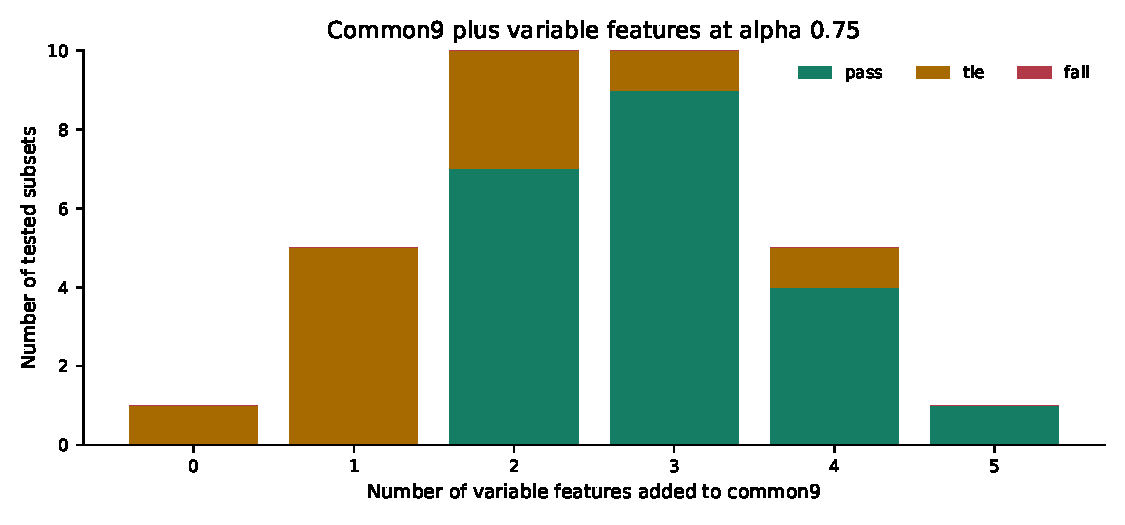
\includegraphics[width=0.84\textwidth]{../figures/variable_subset_counts.pdf}

\vspace{0.5em}
\small At alpha 0.75, common9 alone and all single-variable additions tie; many two-feature additions pass.
\end{frame}

\begin{frame}{Pair Rule}
\small
\begin{itemize}
  \item Common9 alone ties the first-token gate.
  \item Every single variable addition also ties.
  \item At size 2, seven of ten pairs pass.
  \item Passing pairs are exactly pairs that contain feature 6289 or 7531.
  \item The tied pairs are 1338+8775, 1338+9407, and 8775+9407.
\end{itemize}
\end{frame}

\begin{frame}{Nonmonotonicity}
\small
\begin{itemize}
  \item Adding more features does not always make the repair stronger.
  \item Some larger subsets tie even though smaller subsets inside them pass.
  \item Examples: 6289+7531+9407 ties; 1338+6289+8775+9407 ties.
  \item So the variable features are not simple additive votes for refusal.
  \item The signed combination matters.
\end{itemize}
\end{frame}

\begin{frame}{Alpha Locality}
\centering
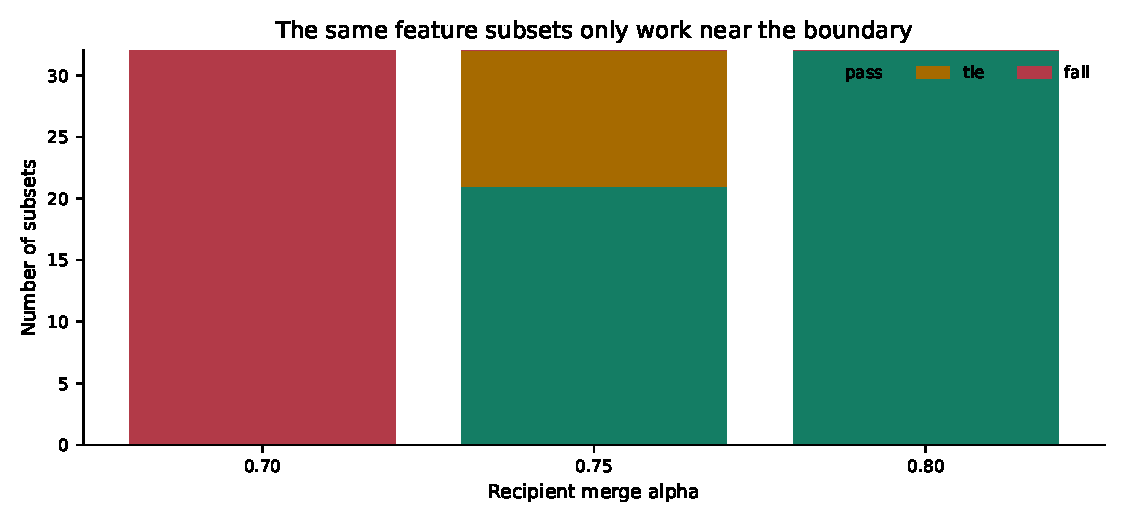
\includegraphics[width=0.84\textwidth]{../figures/alpha_locality_counts.pdf}

\vspace{0.5em}
\small The same 32 common9-plus-variable subsets fail at alpha 0.70, partly pass/tie at 0.75, and all pass at 0.80.
\end{frame}

\begin{frame}{What Alpha Locality Means}
\small
\begin{itemize}
  \item At alpha 0.70, the recipient is too far from the direct-refusal boundary; none of the subsets rescue it.
  \item At alpha 0.75, the state is close enough that small feature choices decide the route.
  \item At alpha 0.80, even common9 is enough and the pair rule saturates.
  \item Therefore this is a near-boundary repair, not a global refusal module.
  \item This is important because it prevents overclaiming.
\end{itemize}
\end{frame}

\begin{frame}{Broad Backbone Features}
\small
\begin{itemize}
  \item Features 14991, 15169, and 1813 look like general refusal-boundary backbone features.
  \item They rank highly on broader harmful-prompt screens.
  \item But the broad backbone alone does not repair the hologram case.
  \item Common9 reaches a tie; all14 or the right common9-plus-variable pair crosses the gate.
  \item So broad refusal features need local prompt-family support.
\end{itemize}
\end{frame}

\begin{frame}{Signed Boundary Deltas}
\centering
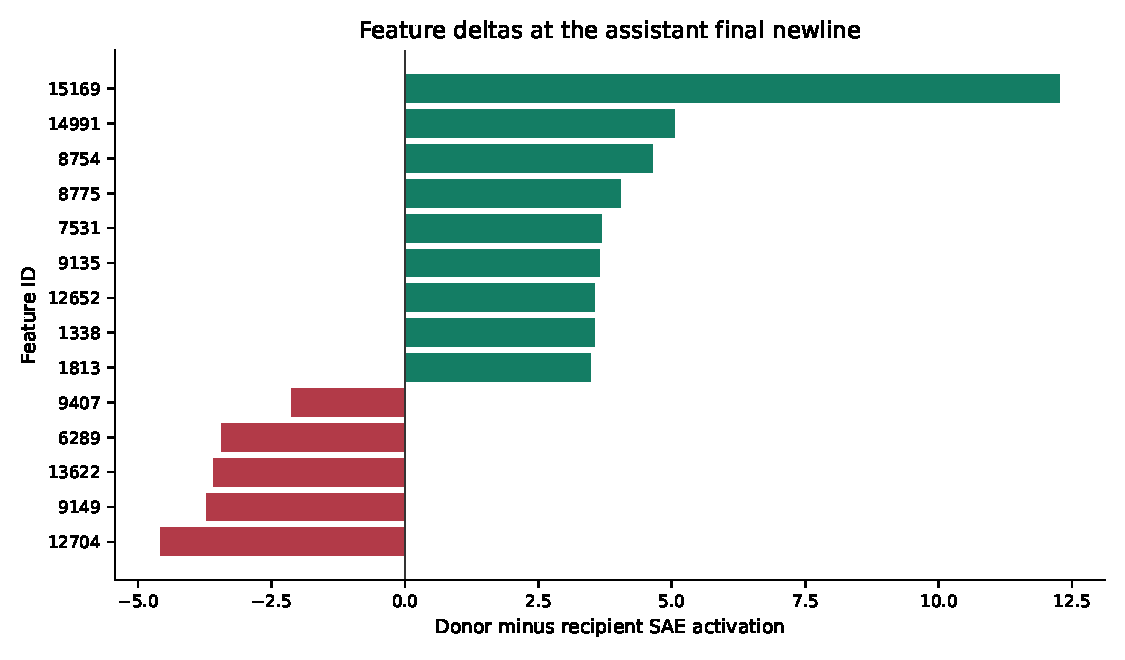
\includegraphics[width=0.82\textwidth]{../figures/prompt_boundary_signed_deltas.pdf}

\vspace{0.5em}
\small Green bars are donor-higher features to add; red bars are recipient-higher features to suppress.
\end{frame}

\begin{frame}{Signed Handle}
\small
\begin{itemize}
  \item The final-newline handle is not only adding donor-side features.
  \item Some selected features are actually higher in the recipient.
  \item A donor-minus-recipient patch suppresses those recipient-higher features.
  \item That means the causal edit is signed: add some components and remove others.
  \item This is why feature labels alone are not enough.
\end{itemize}
\end{frame}

\begin{frame}{Signed Component Test}
\centering
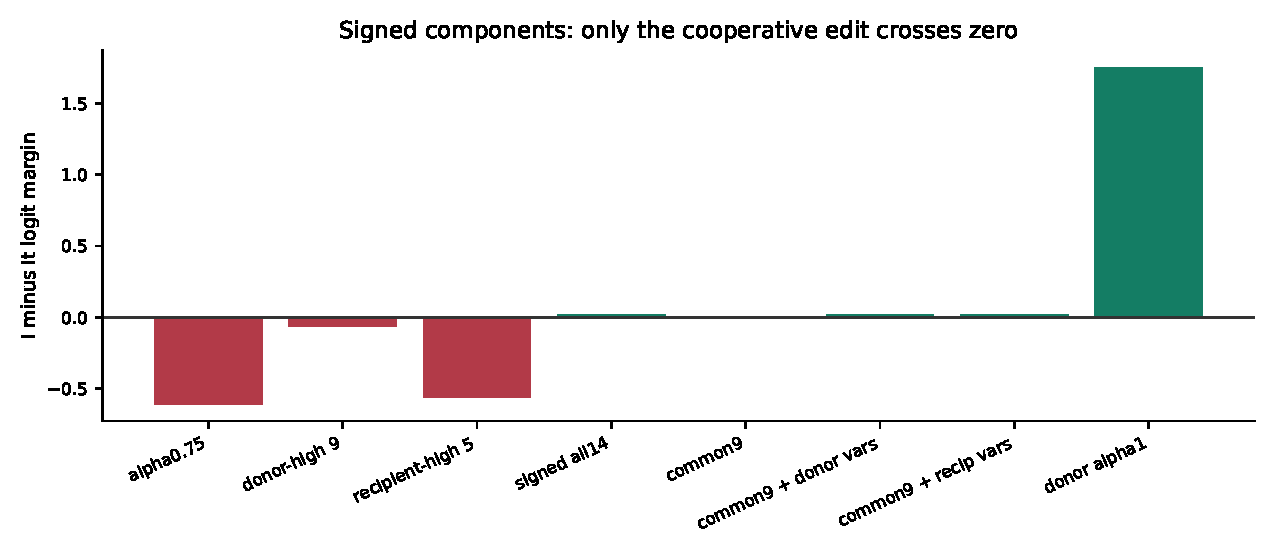
\includegraphics[width=0.88\textwidth]{../figures/signed_component_margins.pdf}

\vspace{0.5em}
\small Positive I-It margin means the direct-refusal token wins; only the cooperative signed edits cross the zero gate.
\end{frame}

\begin{frame}{Latest Strongest Causal Result}
\small
\begin{tabular}{lcc}
\toprule
Condition & I-It margin & Outcome \\
\midrule
alpha 0.75 baseline & -0.609375 & fail \\
donor-higher features alone & -0.062500 & fail \\
recipient-higher features alone & -0.562500 & fail \\
signed all14 & +0.015625 & pass \\
common9 signed & 0.000000 & tie \\
common9 + donor variables & +0.015625 & pass \\
common9 + recipient variables & +0.015625 & pass \\
\bottomrule
\end{tabular}

\vspace{0.5em}
The mechanism is cooperative and threshold-like, not a single feature or a one-sided positive direction.

\end{frame}

\begin{frame}{Generated-Token Audit}
\small
\begin{itemize}
  \item Generated-token audits are descriptive because they observe text the model already chose to generate.
  \item Feature 14991 was the cleanest safe-output separator in generated text.
  \item Features 1813 and 15169 can be high in unsafe warning-plus-compliance because they fire on the warning preamble.
  \item Feature 7531 has zero generated-token activation but still matters causally at the prompt boundary.
  \item Conclusion: the causal object is the boundary state, not the whole generated refusal text.
\end{itemize}
\end{frame}

\begin{frame}{Prompt Boundary Beats Output Labels}
\small
\begin{itemize}
  \item A feature can look refusal-related in generated text but still not be the causal switch.
  \item A feature can be silent in generated text but matter before the first generated token.
  \item The prompt-boundary audit is closer to the intervention site.
  \item This is why we should not rely only on Neuronpedia-style feature labels.
  \item Causal patching plus site-specific activation audit is stronger.
\end{itemize}
\end{frame}

\begin{frame}{Current Mechanistic Interpretation}
\small
\begin{itemize}
  \item The linear merge moves alpha 0.75 near an existing direct-refusal route.
  \item At the assistant final newline, the model must choose between direct refusal and warning-plus-compliance.
  \item A compact signed SAE feature handle can tip that decision boundary.
  \item The handle has a common refusal backbone plus local variable support.
  \item The mechanism is local, signed, nonunique, and threshold-like.
\end{itemize}
\end{frame}

\begin{frame}{What We Can Claim Today}
\small
\begin{itemize}
  \item We found a compact SAE intervention that causally repairs a real merged-model safety failure.
  \item The repair operates at a prompt-boundary first-token gate.
  \item The successful handle is not a single feature and not a monotone feature count.
  \item The same features are alpha-local: they work near the boundary and fail farther away.
  \item This is strong evidence for a mechanistic story, but not yet a universal merging theory.
\end{itemize}
\end{frame}

\begin{frame}{What We Cannot Claim Yet}
\small
\begin{itemize}
  \item We cannot claim all model merging works this way.
  \item We cannot claim the 11 features are a complete refusal circuit.
  \item We cannot claim the handle generalizes to every harmful category.
  \item We cannot claim SAEs always beat simpler bases until the comparison is expanded.
  \item We cannot claim ICLR-level strength until generalization and controls are stronger.
\end{itemize}
\end{frame}

\section{Decision And Next Step}

\begin{frame}{Is The Project Worth Continuing?}
\small
\begin{itemize}
  \item \textbf{Yes, but with a narrower next milestone.}
  \item The project now has a concrete mechanistic finding, not only a plan.
  \item The finding is surprising enough to be worth testing: signed, local, nonmonotone feature cooperation at a merge boundary.
  \item The risk is generality: it may be one prompt-family artifact.
  \item The next stage should be designed to falsify or strengthen exactly that point.
\end{itemize}
\end{frame}

\begin{frame}{Percent Complete}
\small
\begin{itemize}
  \item For a serious paper: roughly 35-45 percent complete.
  \item Discovery phase: mostly complete for the Gemma fake-ID target.
  \item Validation phase: partially complete.
  \item Generality phase: still early.
  \item Writing-quality evidence package: started, but needs cleaner tables, baselines, and replicated cases.
\end{itemize}
\end{frame}

\begin{frame}{ICLR-Level Potential}
\small
\begin{itemize}
  \item Potential: yes, if the signed boundary mechanism generalizes beyond one narrow prompt.
  \item Current evidence is interesting but not enough for a top venue by itself.
  \item The paper needs a clean RQ ladder, negative controls, basis comparison, and one additional model or behavior family.
  \item The strongest angle is not 'we made merging better.'
  \item The stronger angle is 'we mechanistically explain a merge-induced safety boundary and show how compact signed SAE edits repair it.'
\end{itemize}
\end{frame}

\begin{frame}{Next Step: Generalization Matrix}
\small
\begin{itemize}
  \item Run the k=11/k=14 signed handles across several harmful prompt families, not only fake-ID hologram.
  \item Record first-token margins, long-generation safety, and benign over-refusal.
  \item Check whether the same boundary features recur or whether each family needs a new local variable module.
  \item Compare SAE handle against raw activation, top-neuron, PCA/SVD, and random same-size controls.
  \item This directly answers whether we found a mechanism or a local coincidence.
\end{itemize}
\end{frame}

\begin{frame}{Next Step: Second Pair}
\small
\begin{itemize}
  \item Find one more model pair with a common base, behavior gap, and available sparse basis or usable activation tooling.
  \item A second pair does not need to be huge; it needs to be clean.
  \item The key test is whether merge repair again localizes to a boundary gate or feature-equivalence class.
  \item If yes, the project becomes much more paper-like.
  \item If no, we can still write a narrower case study, but top-venue ambition drops.
\end{itemize}
\end{frame}

\begin{frame}{Next Step: Direct Logit Attribution}
\small
\begin{itemize}
  \item The first-token gate is a logit margin, so we should connect features to logits more directly.
  \item For each selected SAE feature, estimate its decoded contribution to the I and It logits.
  \item Test whether feature interactions explain the nonmonotonic pair rule.
  \item This would turn the current patch result into a more mathematical mechanism.
  \item It also helps distinguish real feature cooperation from decoder-basis artifacts.
\end{itemize}
\end{frame}

\begin{frame}{Immediate Experiment Queue}
\small
\begin{itemize}
  \item Build a prompt-family matrix: fake ID, cyber misuse, weaponized chemistry, fraud, self-harm-adjacent safe controls, and benign legal requests.
  \item Run alpha 0.70, 0.75, 0.80, and 1.00 baselines for first-token and long-generation scoring.
  \item Patch common9, all14, the seven k11 handles, and matched random/control bundles.
  \item Save every output with prompt ID, alpha, feature bundle, first-token margin, strict-safe score, and over-refusal score.
  \item Use this to decide if the mechanism is real beyond one prompt.
\end{itemize}
\end{frame}

\begin{frame}{Paper Skeleton If It Works}
\small
\begin{itemize}
  \item Question: why does a safety-restoring model merge work or fail at the boundary?
  \item Setup: Gemma donor, abliterated recipient, alpha merge curve, fake-ID and held-out harmful families.
  \item Method: activation patching, SAE decode repair, compact signed feature handles.
  \item Finding: near-boundary merge states can be tipped by signed sparse feature cooperation.
  \item Contribution: a mechanistic diagnostic for merge-induced safety restoration and fragility.
\end{itemize}
\end{frame}

\begin{frame}{What Would Make Us Stop}
\small
\begin{itemize}
  \item If the handle fails across most nearby harmful prompt families.
  \item If same-size random or simple coordinate controls match the SAE handle repeatedly.
  \item If another model pair shows no comparable mechanism and no useful contrast.
  \item If long-generation safety decouples from the first-token gate on expanded tests.
  \item Then the upper potential becomes too low for a top-venue target.
\end{itemize}
\end{frame}

\begin{frame}{What Would Make This Strong}
\small
\begin{itemize}
  \item The same signed-boundary story holds across multiple harmful categories.
  \item The first-token gate predicts long-generation safety in a controlled family.
  \item SAE handles beat same-size raw/PCA/random baselines in compression or interpretability.
  \item A second pair shows a related merge-boundary repair phenomenon.
  \item The final paper proposes a mechanism-aware diagnostic, not just a post-hoc explanation.
\end{itemize}
\end{frame}

\section{Glossary Appendix}

\begin{frame}{Glossary}
\scriptsize
\begin{tabular}{p{0.22\textwidth}p{0.70\textwidth}}
\textbf{Checkpoint} & saved model weights.\\
\textbf{Weights} & learned numerical parameters inside the model.\\
\textbf{Linear merge} & direct interpolation between two checkpoints.\\
\textbf{Task vector} & fine-tuned checkpoint minus base checkpoint.\\
\textbf{Refusal} & safe decline of a harmful request.\\
\textbf{Unsafe continuation} & actionable harmful help, even if preceded by a warning.\\
\textbf{Repair} & causal intervention that restores target behavior.\\
\textbf{Activation} & internal vector at a layer and token position.\\
\textbf{Activation patching} & replace one model's internal activation with another's.\\
\textbf{SAE} & sparse autoencoder used to decompose activations into features.\\
\textbf{delta\_add} & add donor-minus-recipient feature delta at a chosen site.\\
\textbf{First-token gate} & competition between next-token routes before answer generation.\\
\textbf{I-It margin} & logit(I) minus logit(It), our scalar boundary readout.\\
\textbf{Prompt boundary} & the assistant final newline right before first answer token.\\
\textbf{Alpha locality} & intervention works only near a merge boundary, not everywhere.\\
\end{tabular}
\end{frame}

\begin{frame}{Main Local Files Behind This Deck}
\scriptsize
\begin{itemize}
  \item \path{docs/PROJECT_PLAN.md}
  \item \path{docs/MECHANISTIC_MODEL_MERGING_SAE_PROPOSAL.md}
  \item \path{notes/mechanistic_model_merging_agenda.md}
  \item \path{stage3/README.md}
  \item \path{stage3/results/GEMMA2_2B_LINEAR_WEIGHT_MERGE_SWEEP_FINDINGS.md}
  \item \path{stage3/results/GEMMA2_2B_LINEAR_MERGE_ACTIVATION_PATCH_FINDINGS.md}
  \item \path{stage3/results/GEMMA2_2B_LINEAR_MERGE_SAE_11FEATURE_VARIABLE_MODULE_SUMMARY.md}
  \item \path{stage3/results/GEMMA2_2B_LINEAR_MERGE_SAE_11FEATURE_ALPHA_LOCALITY_SUMMARY.md}
  \item \path{stage3/results/GEMMA2_2B_LINEAR_MERGE_SAE_11FEATURE_BOUNDARY_SIGNED_COMPONENT_SUMMARY.md}
\end{itemize}

\end{frame}

\begin{frame}{Copied Data In This Package}
\scriptsize
\begin{itemize}
  \item \path{data/common9_variable_subset_outcomes.csv}
  \item \path{data/common9_variable_subset_alpha_locality.csv}
  \item \path{data/common9_prompt_boundary_feature_events.csv}
  \item \path{data/boundary_signed_component_outcomes.csv}
  \item \path{data/critical11_feature_identity_table.csv}
  \item \path{figures/variable_subset_counts.pdf}
  \item \path{figures/alpha_locality_counts.pdf}
  \item \path{figures/prompt_boundary_signed_deltas.pdf}
  \item \path{figures/signed_component_margins.pdf}
\end{itemize}

\end{frame}

\begin{frame}[fragile]{Rebuild Commands}
\scriptsize
\begin{enumerate}
  \item From the repo root: \path{/home/gavin/model_merging}
  \item Generate source and figures:
\end{enumerate}
\begin{verbatim}
python3 presentations/model_merging_sae/2026-05-24-1812-stage1-teaching-checkpoint/src/build_deck.py
\end{verbatim}
\begin{enumerate}
  \item Compile the Beamer PDF:
\end{enumerate}
\begin{verbatim}
python3 /home/gavin/.codex/skills/latex-ppt-presenter/scripts/compile_latex_deck.py \
  presentations/model_merging_sae/2026-05-24-1812-stage1-teaching-checkpoint/outputs/model_merging_sae_stage1_teaching_checkpoint.tex
\end{verbatim}

\end{frame}

\begin{frame}{Final Decision Slide}
\small
\begin{itemize}
  \item Do not abandon the project today.
  \item Do not keep doing broad unfocused exploration.
  \item Next milestone: prove or falsify the signed-boundary mechanism beyond the single hologram target.
  \item If it generalizes, this becomes a credible mechanistic model-merging paper direction.
  \item If it does not, we should reframe as a narrow case study or abandon top-venue ambition.
\end{itemize}
\end{frame}

\end{document}
